\chapter{相关工作}

本章节首先介绍大模型推理相关概念和工作,包括对现有流行大模型的架构和算子的介绍,对推理加速的技术尤其是模型量化的相关工作进行介绍,以及阐明推理性能和矩阵向量乘算子的关系。其次介绍近存计算的研究现状,首先介绍近存计算的发展历史以及相关工作,然后介绍第一款商用近存计算硬件UPMEM的硬件架构和特性,最后详细介绍各个领域基于UPMEM加速应用的相关工作。

\section{大模型推理介绍}

\subsection{基本概念}
自2022年11月OpenAI发布聊天机器人产品ChatGPT以来,其强大的语言理解对话能力和逻辑推理能力震惊了世界,并以势不可挡之式席卷全球,并受到了资本的热捧。其背后拥有强大智能的GPT大语言模型凭借惊人的通用智能应用到了各行各业,开启了“LLM时代”。

GPT模型的结构源于Google在2017年提出的一个基本模型结构Transformer \cite{Transformer}。Transformer模型本身是为解决序列到序列(Seq2Seq)的自然语言翻译问题,构造了编码器(Encoder)模型用于理解待翻译序列,再使用解码器(Decoder)模型结合Encoder的理解生成翻译序列。在Encoder和Decoder中创造性地使用了自注意力(Self-Attention)机制,使得模型的性能表现异常优异,击败了当时其他的翻译模型。基于Transformer结构,自然语言处理(Natuarl Language Processing,NLP)领域的模型逐渐形成了三条不同的发展路径,分别是Encoder-Only架构、Encoder-Decoder架构和Decoder-Only架构。Encoder-Only架构的模型非常擅长做语义理解,其应用领域往往是文本分类,其中最著名的模型当属Bert\cite{Bert};Encoder-Decoder架构和Transformer的应用领域类似,主要是用在机器翻译领域,其中比较著名的模型同是Google公司的T5\cite{T5}。Bert和T5模型在前GPT时代基本确定了NLP模型的预训练+微调的部署范式:由大公司使用大量数据集训练基础通用模型(预训练模型),在此基础上由使用者自行用少量高质量数据微调模型以适应不同的下游任务。

\begin{figure}[!htbp]
	\centering
    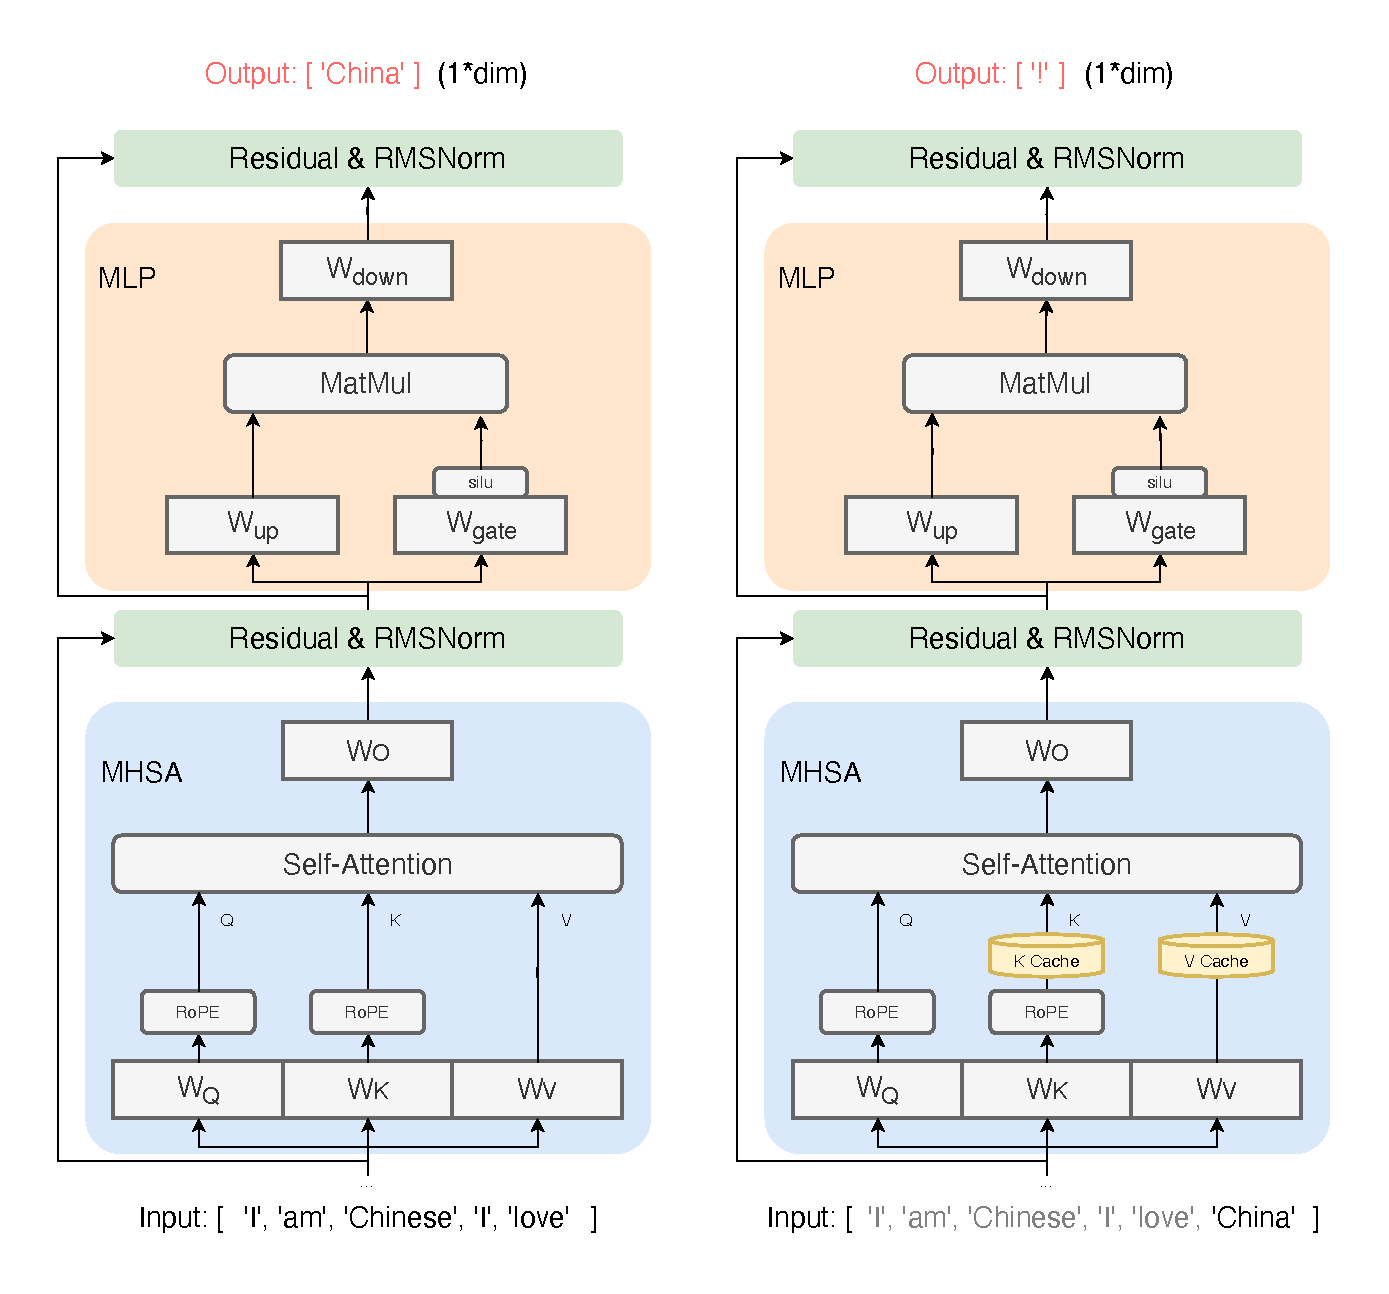
\includegraphics[width=0.9\textwidth]{figures/LLMInfer.pdf}
	\caption{现代主流大模型推理的两个阶段}
    \label{LLMInfer}
\end{figure}

Decoder-Only架构的模型与前面两者不同,可以直接自回归地生成自然语言,常常应用到文本续写领域和聊天机器人,其中代表模型就是OpenAI的GPT模型。最早的GPT-1\cite{GPT-1}仍然采用有监督和无监督混合训练的方式直接生成下一个词元,效果并不是很理想。到了GPT-2\cite{GPT-2},GPT模型开始使用无监督的训练方式,加大了训练数据量并提升模型参数规模到150亿,无须微调模型而只需简单地通过写提示词(Prompt)就可以达到非常好的效果。到了GPT-3\cite{GPT-3},进一步将模型参数量提升到了惊人的1750亿,并专注于提升模型的上下文学习能力(In-Context-Learning,ICL)。量变引起了质变,GPT-3的效果非常优异,为接下来的GPT3.5以及ChatGPT的爆火做了铺垫。得益于Decoder-Only架构模型在大量数据集上的良好零样本(Zero Shot)学习能力\cite{Zero-Shot}和少样本(Few Shot)微调能力\cite{Few-Shot},大模型的参数规模不断增长(从前GPT时代Bert的1.1亿参数到GPT-3的1750亿),参数量的膨胀对于大模型推理提出了严峻的挑战,大公司旗下的云计算中心需要使用集群分布式推理上千亿大模型,常见的硬件几乎无法部署推理参数量最小的70亿参数模型。

要想了解大模型在常用硬件平台上的推理瓶颈,就需要先了解大模型的结构,从开源的大模型入手是最佳选择。其中使用最广微调性能最高的开源大模型当属Facebook推出的Llama系列。Llama系列的模型架构都秉承类似的结构,以Llama2-7B\cite{Llama2}为例,模型一般由多层Decoder组成,每层Decoder分为多头注意力(Multi-Head Self-Attention,MHSA)和前馈神经网络(Feed-Forward Neural Network,FFN)两个主要部分。在LLM进行推理的时候,分为两个阶段:用户输入提示词(Prompt)进入网络到模型生成第一个token的阶段称作预填充阶段(The Prefilling Stage),再生成了第一个token之后,LLM不断自回归生成下一个token直到输出终止符的阶段称为解码阶段(The Decoding Stage)。如图\ref{LLMInfer}所示,两个阶段执行的计算并不相同,主要体现在Self-Attention部分,预填充阶段执行的是GEMM,而在解码阶段执行的是GEMV。两者不同的原因主要在于现代Decoder-Only架构的LLM在自回归生成阶段普遍采用因果注意力(Causal Self-Attention)并通过KVCache机制减少计算量,如图\ref{KVCache}所示,因果注意力会使用因果掩码对QK乘积矩阵的上三角置0:当生成第四个token时,Query1和Key2到Key4点注意力都被掩码置0无效化,为的是防止其与未来生成的token做注意力计算以保持因果一致性。第四个token进行推理时真正的新数据就是Query4、Key4、Value4和Attention4。因而KVCache就是将K向量和V向量缓存起来,每次只需要最新生成的Query向量参与运算,减少重复的注意力计算,此时Self-Attention的计算为GEMV。

\begin{figure}[!htbp]
	\centering
    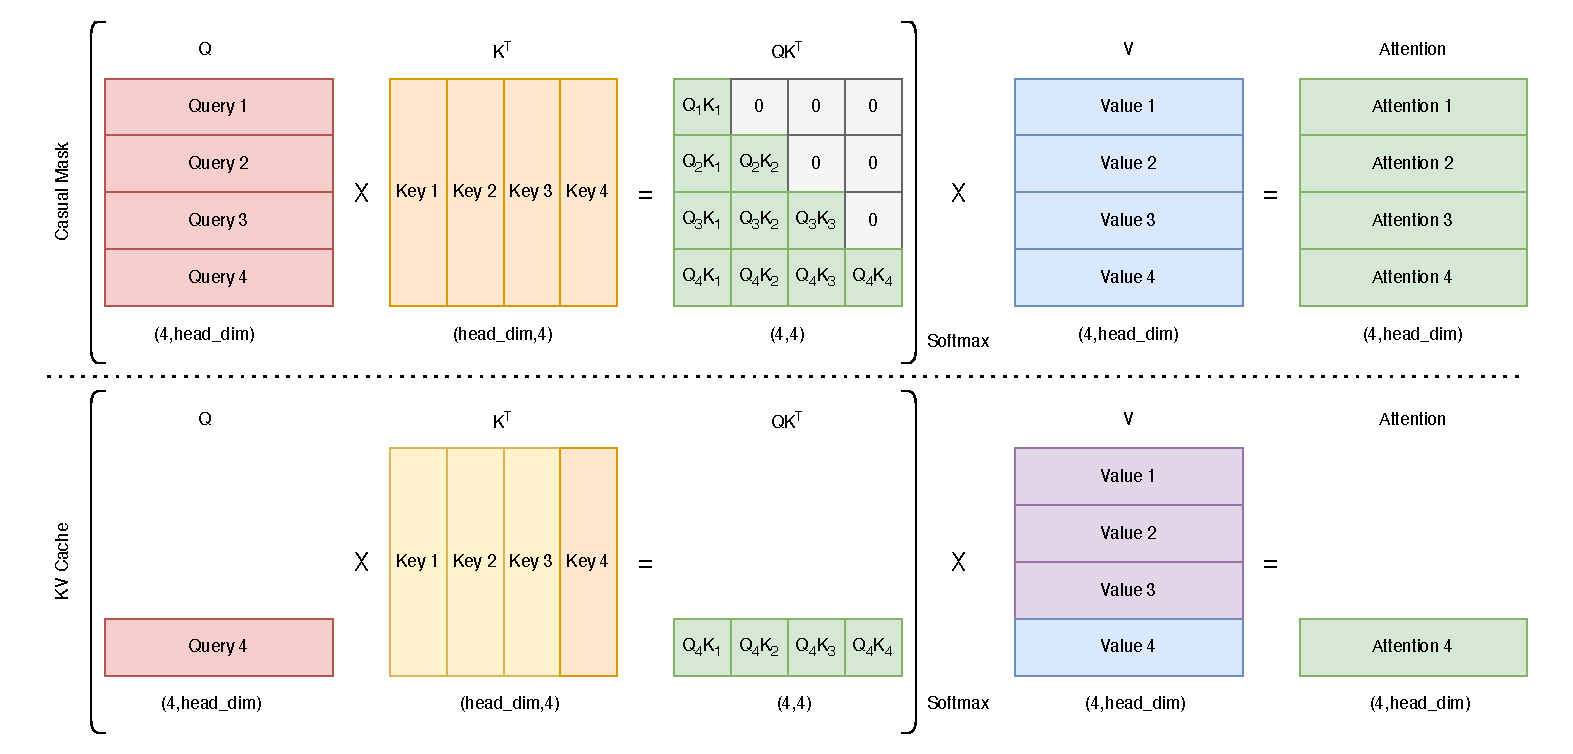
\includegraphics[width=0.9\textwidth]{figures/KVCache.pdf}
    \caption{基于因果掩码和KV缓存的自注意力机制}
	\label{KVCache}
\end{figure}

大模型的推理往往表现为内存瓶颈,尤其是在用户量不多的本地或边端场景,推理中的解码阶段占据主导地位\cite{InferLinear},有数据表明,解码阶段代表性算子GEMV平均占据82.3\%的GPU运行时间,而预填充阶段的代表性算子GEMM的平均耗时只占2\%,剩下的一些非线性算子总占比不到20\%;同时在执行GEMV算子时,GPU的硬件利用率显著地低于GEMM算子,并且将绝大部分的时间消耗在内存拷贝和数据传输上,表现为内存瓶颈\cite{SamsungHotChips}。这使得缓解内存数据的搬移成为大模型推理的主要性能瓶颈,针对GEMV的优化对于提升大模型的推理效率至关重要,具有重大研究价值。

\subsection{大模型量化技术}
加速大模型推理有许多手段,包括模型量化、模型压缩、矩阵稀疏化、知识蒸馏、内存管理和批处理等等技术\cite{LLMInferSurveyTsingHua},其中最流行以及能够显著降低模型的内存瓶颈的方法当属模型量化。所谓的量化就是指将模型的高bit参数(float32)通过一系列措施(最小化推理精度损失)转化为较低的位宽存储。这样做能够极大缩减模型尺寸,在硬件资源有限的情况下支持低精推理,使得本地大模型或边端大模型成为可能。以一组float32向量量化成int8向量为例,如图\ref{Quant:Norm}所示,取得这组float32向量的最大绝对值5.4,将其映射到int8的动态范围$[-128,127]$,计算得到缩放因子scale为23.5,将向量的每个元素与scale相乘并做整数舍入得到int8向量,此时完成量化;当需要量化后的向量参与计算时需要先解量化,将int8向量的每个元素与scale相除进行解量化,还原成float32向量。

\begin{figure}[htbp!]
	\centering
    
	\subfigure[正常对称量化]{
		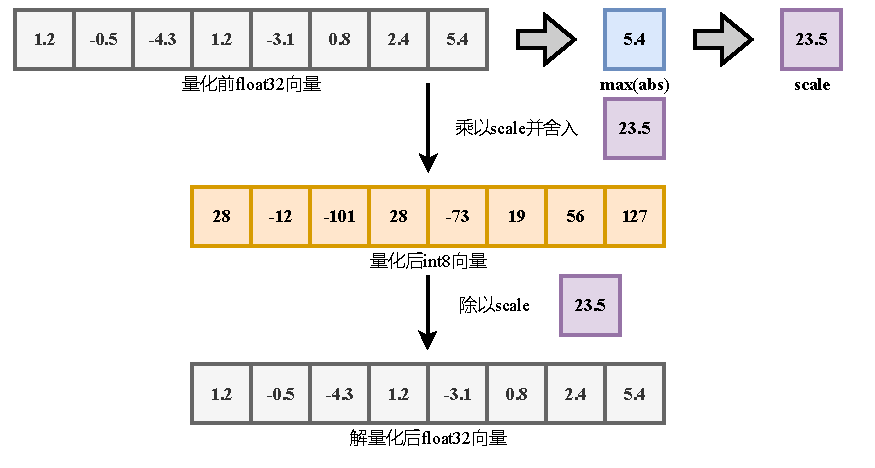
\includegraphics[width=0.45\textwidth]{figures/QuantNorm.pdf}
		\label{Quant:Norm}}
	\subfigure[含有离群值的量化]{
		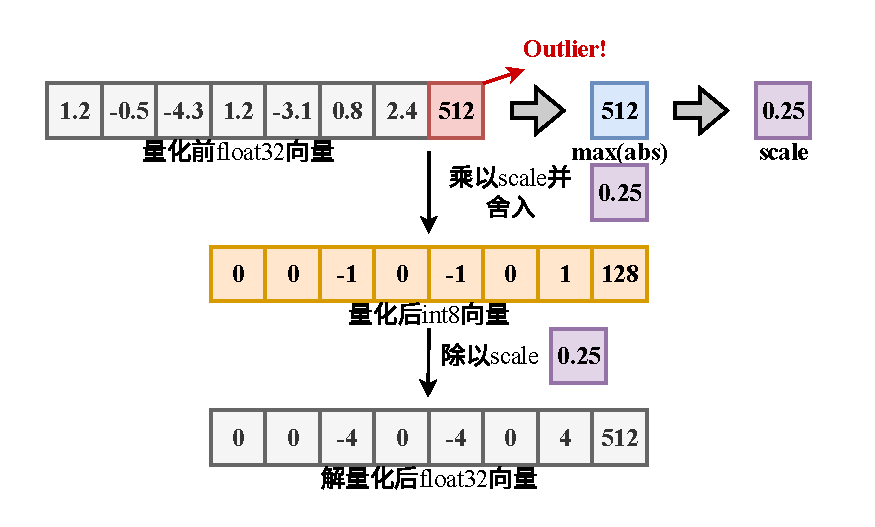
\includegraphics[width=0.45\textwidth]{figures/QuantAbnorm.pdf}
        \label{Quant:Abnorm}}
	\label{Quant}
	\caption{32位浮点数向量对称量化为8位定点数}
\end{figure}

上述量化是非常标准的对称量化:所谓对称量化就是取得原数值域的一个对称区间量化到目标数值区域,一般使用最大绝对值确定对称区间。而与之相对的非对称量化就是量化原数值域的非对称区间,使用的是最小值和最大值;对称量化是非对称量化的一种特殊情况,二者都可以用公式\ref{QuantEqu}来表示,其中r是原始浮点数,S是缩放因子scale,Z是零点偏移,q是量化后的数值。当为对称量化时,零点无偏移,$r_{max}-r_{min}=2r_{max_abs}$。量化一般采用训练后量化(Post Training Quantization,PTQ)的方式以降低量化成本(简单的数学变换或者少量校准数据集),主要的量化对象就是激活值和权重,按照上述的方式将激活和权重全部量化到8bit的量化称为W8A8(weight 8bit activation 8bit)量化。但是假如激活向量或权重矩阵中,存在一个特别大的值如图\ref{Quant:Abnorm}所示,为512,那么scale计算就得到为0.25,将原float32向量与scale相乘再舍入取整为int8,发现绝大部份数都变为了0,0在浮点数制中是一个特殊值,任何数与0相乘或相除都是0,因此将int8向量反量化后,float32向量中的大部分数据也都变为0,从而导致精度严重损失。

\begin{equation}
    q = round\left(\frac{r}{S} + Z\right), \quad S=\frac{r_{max}-r_{min}}{q_{max}-q_{min}}, \quad Z=q_{min}-\frac{r_{min}}{S}
    \label{QuantEqu}
\end{equation}

为了解决这种离群值带来的量化精度影响,许多工作提出了不同的方案。其中比较出名的int8量化方案为Dettmers等人提出的LLM.int8\cite{LLMINT8},该方法的主要思路在于离群值分布往往在特定的维度且比较稀疏,因此可以将离群值提取出来用float16进行计算,剩下的量化到int8,这样的混合精度分解能够很大程度提升量化精度。SmoothQuant采用了不同的思路\cite{SmoothQuant}做W8A8量化,其观察到当前的LLM的激活相对权重难以量化,因此提出了一种数学上等价的逐通道缩放变换,引入一个对角矩阵存放激活逐通道的缩放因子scale factor,将原激活除以对应的缩放因子作为新的激活,原矩阵等价地乘以对应的缩放因子作为新的权重,这样就能将激活中难以量化的离群值平滑到了权重当中,二者都变得容易量化了。Lin等人提出了一种W4A16的量化(仅量化权重)\cite{AWQ},其核心思想是基于激活值的分布挑选对最终结果影响较大的权重,将这些显著权重保留精度分解,剩余权重采用低bit量化,以较小的量化误差达到大幅度减少内存占用的效果。在量中同样有一类工作可以实现非常低bit的量化,即基于机器学习的量化,其中最具代表性的当属GPTQ。GPTQ\cite{GPTQ}本身的核心思想是对LLM进行逐层量化,希望在该层找到一个新权重(量化过后),使得其和使用老权重相比输出之间的误差尽可能小。GPTQ将这个作为训练目标使用机器学习的方式进行优化,基于此前的OBQ工作\cite{OBQ},对训练算法做了近似和加速,能够达到3-4bit的超低精度量化。Yao等人开展了一系列LLM上的量化工作:ZeroQuant系列\cite{ZeroQuant1,ZeroQuant2,ZeroQuantFP}。ZeroQuant-V1主要是针对GPU硬件构建了强大的推理后端并使用逐层知识蒸馏缓解量化带来的精度下降问题\cite{ZeroQuant1};ZeroQuant-V2则是针对常见的不同的PTQ方法进行了全面的分析,并提出了一种低秩补偿的技术来缓解量化带来的误差\cite{ZeroQuant2};ZeroQuantFP基于GPTQ的量化和低秩补偿,重点探索来浮点数据格式对于量化的影响,得出float8激活优于int8,float8权重与int8权重相当,float4权重优于int4权重的结论\cite{ZeroQuantFP}。

\subsection{矩阵向量乘算子}
GEMV作为基本的线性代数运算被广泛地使用于各种科学计算和神经网络计算当中,其本身可以视作GEMM中矩阵维度为1的一种特例。关于GEMM和GEMV的计算加速优化方法一直是研究人员的研究热点,因为GEMM和GEMV作为BLAS(Basic Linear Algebra Subprograms)中最为基本的两个,其性能的提升将极大提升建立于其基础上的应用性能。GEMM的优化主要分为两个方面,分别是数学算法上的优化和计算机系统层面的优化。前者主要是在数学算法上减少GEMM需要执行计算量,其中最经典的算法是Strassen算法\cite{Strassen},其将相乘的每个矩阵分别分解为大小相同的四个子矩阵,通过对四个子矩阵执行一系列的矩阵加法和乘法运算得到最终的乘积矩阵,成功将矩阵乘法的时间复杂度从$\O(n^3)$优化到$\O(n^{\log_{2}7})$,但是由于GEMV中向量无法进行有效地分块,因此Strassen算法无法直接应用到GEMV上的优化;另一种,也是工作最多且更加有效的优化,通过将矩阵进行合适的分块和内存布局,减少计算机在执行计算过程中的重复的和开销大的访存,增强数据的局部性。常见的工作都是根据所使用硬件的离计算核心最近的一级存储器件(比如CPU中是L1 Data Cache,GPU中CUDA的shared memory\cite{Cuda})的存储大小,对矩阵进行合适大小的分块以在执行每个小块的计算时访存都能落到最近的存储器而无需访问更低速的内存。

GEMV的常规计算方式有两种,如图\ref{GEMVBasic}所示,可以类似向量的内积和外积定义GEMV的内积和外积概念。如图\ref{GEMVBasic:Inner},GEMV的内积可以定义为向量和矩阵的一行或一列的对应元素乘积之和,结果是最终结果向量的一个元素。如图\ref{GEMVBasic:Outer},GEMV的外积可以定义为向量的某个元素与矩阵对应行或列的所有元素乘积,结果是一个向量,将所有向量对应相加得到最终结果向量。在传统CPU平台下,GEMV的内积效率更高,因为其数据局部性更好,内积的累加结果基本能够留存在寄存器中,不需要频繁读写结果向量;当然GEMV的外积在某些场景下也有用武之地。除了考虑寄存器效率外,高速缓存(Cache)的命中率也非常重要:无论是何种方式,只需要Cache容量大于矩阵的两行或两列所占的空间,命中率就会很高,如果矩阵的两行或两列所占的空间过大,则需要将矩阵或向量在某一个维度上进行分块,以达更高缓存命中率。分块后,对于大多数的存储器来说,顺序读取效率是最高的,因此需要将数据按照顺序访问的方式进行重排,称为数据打包。如\ref{GEMVBasic}所示,将矩阵按行或列分成了N块,对每一块进行数据打包依次计算。

\begin{figure}[htbp!]
	\centering
	\subfigure[GEMV内积]{
		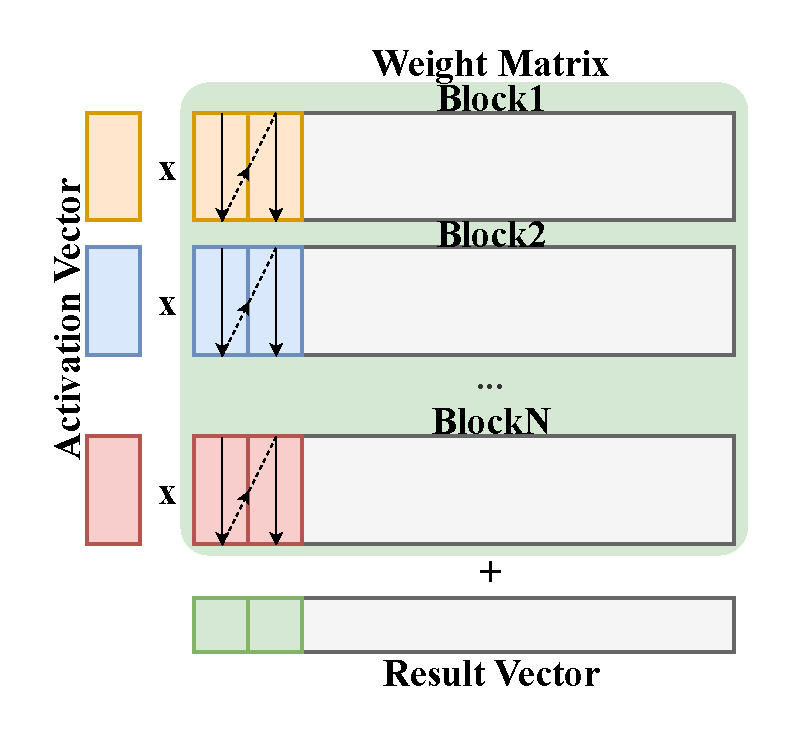
\includegraphics[width=0.43\textwidth]{figures/GEMVInner.pdf}
		\label{GEMVBasic:Inner}}
	\subfigure[GEMV外积]{
		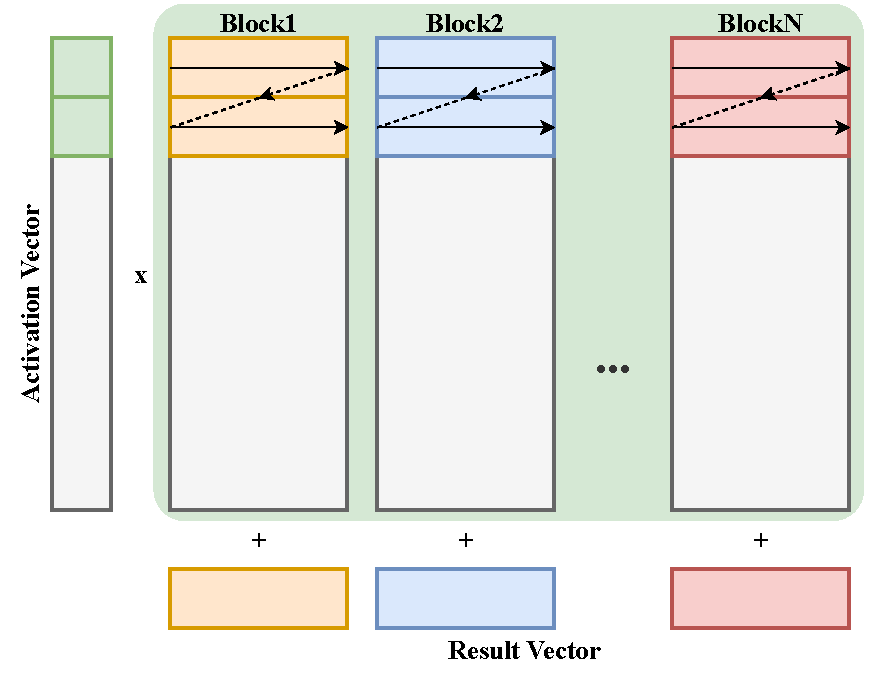
\includegraphics[width=0.47\textwidth]{figures/GEMVOuter.pdf}
        \label{GEMVBasic:Outer}}
	\label{GEMVBasic}
	\caption{矩阵向量乘基本优化方法}
\end{figure}

常规的优化手段如上所述,当然还可以使用多线程进行优化,此时只需要考虑各个线程的数据划分和线程间的同步开销即可。除此之外许多相关硬件被设计并对其加速提供了支持,这其中包括基于单指令多数据(Single Instruction Multiple Data,SIMD)的Intel的向量单元和AVX指令集,可以在0.5个周期内完成512bit向量的融合乘加运算(Fused Multiply Accumulate,FMA)操作\cite{IntelAVX}。还有Nvidia基于单指令多线程(Single Instruction Multiple Threads,SIMT)模型设计的CUDA Core\cite{Cuda},以及专门用于GEMM计算的Tensor Core\cite{TensorCore}等等,都极大地提升了GEMM和GEMV的计算效率。

\section{近存计算研究现状}

\subsection{近存计算技术发展}
早在上世纪七十年代左右,近存计算的思想就已经\cite{CellularLogicInMemory,LogicInMemory}初具雏形,这时普遍提到的概念是“Logic-in-Memory”,其核心思想是在动态随机存取存储器(Dynamic Random Access Memory,DRAM)的存储单元上增加简单的逻辑电路使得DRAM本身可以进行一些简单的运算。在九十年代,Wulf等人针对处理器(CPU)和存储器(DRAM)之间不断增大的速度差异,通过科学的建模和实验进行了分析,通过系统性的分析和实验,提出了内存墙(Memory Wall)的概念以说明CPU和DRAM之间速度存在的难以逾越的鸿沟\cite{MemoryWall}。许多学者围绕该问题提出了不同的解决方案,其中,有部分学者提出存内计算(Processing in Memory, PIM)的思想,希望通过在存储器原地进行计算从而减少CPU的访存以达到更高的性能和更低的能耗。同年就有工作\cite{MicroArchitecturePIM},该结构通过在存储阵列旁加了一些计算单元 (例如 ALU), 用于支持存储阵列内部的数据处理。又如RowClone这篇工作\cite{RowClone}提出在DRAM的同一存储体(Bank)内同时打开多行并利用共享的行缓存器(Row Buffer)实现行之间的快速复制,这种复制无需CPU参与数据搬移,大大提升了复制的效率。此外还有Seshadri等人\cite{BitAndOr,Ambit}的一系列工作,通过利用内存单元本身的模拟特性以及对感应放大器(Sense Amplifier)的简单修改,实现了大批量的按位与(AND)、或(OR)、非(NOT)逻辑操作,由于计算完全发生在DRAM内部,因此不占用内存带宽,可以达到非常高的吞吐。

尽管还有相当一部分此类的工作被提出,但是时代的局限性使得PIM的工作难以落地。一方面是当时的制造工艺无法在内存芯片内集成较为复杂的逻辑单元。另一方面,在内存墙概念被提出的九十年代,互联网的数据量远不如现在庞大,没有弃用原先普通内存,更换造价更加相较高昂PIM型内存的迫切需求\cite{NDPWorkshop}。

本世纪10年代以来,人类社会进入大数据时代,数据量呈现指数级爆炸,而且由于人工智能的兴起,数据密集型场景逐渐增多,大量且频繁数据搬移造成的高延迟和高能耗等问题日渐凸显:跨内存层次结构移动数据的能耗将比执行双精度浮点运算的成本高出两个数量级\cite{EnergyCost}。想要消除这种不必要开销的迫切需求日益增长,计算机系统逐渐从以计算为中心的架构向着以数据为中心的架构发展。此时存内计算被重新提出,其与存储侧计算的思想与大数据时代信息处理的特征不谋而合,重新受到了研究人员的青睐。

与此同时,硬件方面的新进展为存内计算的复兴提供了坚实的土壤——3D堆叠技术(3D-Stacking)的出现极大程度上解决了此前PIM的逻辑集成难题,使得在同一块面积的芯片上集成更复杂高效的逻辑单元成为可能。如图\ref{3DStack}所示,3D堆叠技术纵向堆叠内存芯片,形成多层结构。3D堆叠的内存立方体在最底层集成逻辑层,为存储侧计算单元提供设计空间,逻辑层上方即是堆叠的存储层。层与层之间通过硅穿孔(Through-Silicon Vias, TSV)TSV形成垂直互联。TSV能够高效传输数据,同时一个存储立方可能包含大量的TSV进行垂直互联,因而可以提供极大的内部存储带宽。凭借着新硬件技术,Ahn等人\cite{Tesseract}提出Tesseract使用3D堆叠技术加速大规模的图处理。

\begin{figure}[!htbp]
	\centering
    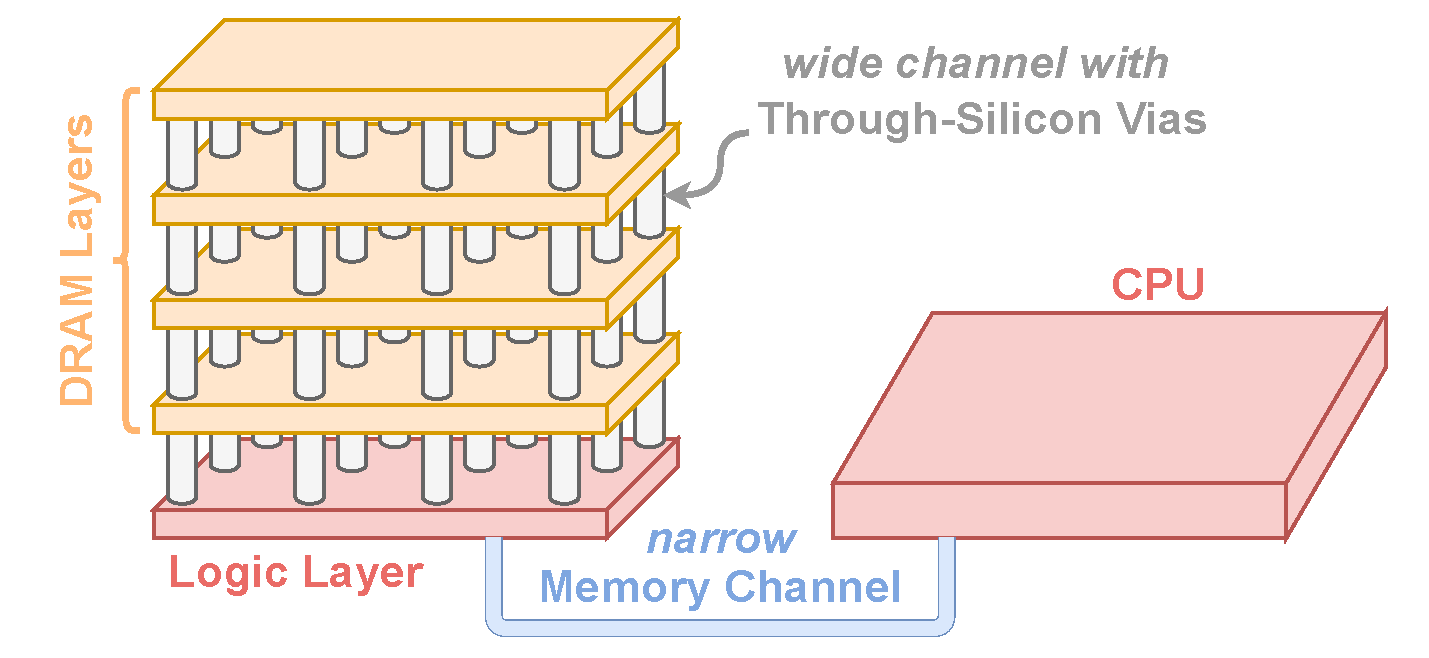
\includegraphics[width=0.9\textwidth]{figures/3DStack.pdf}
    \caption{3D堆叠内存结构}
	\label{3DStack}
\end{figure}

与此同时由于人工智能(Artificial Intelligence,AI)的兴起,许多专用于神经网络的PIM加速芯片也被设计出来,其中较为著名的就是三星的HBM-PIM(High Bandwidth Memory,HBM)产品\cite{SamsungHBMPIM},该产品采用20nmDRAM工艺,使用3D堆叠技术堆叠封装了4层裸芯(Die),每层die的bank组内增加了专门用于做16位浮点数乘加操作的PIM单元以处理神经网络中的矩阵操作。此外三星的另一个产品AxDIMM\cite{AxDIMM}也采用了近存计算的技术,其将DRAM芯片(Chip)和一块FPGA处理单元整合到一块有着DDR4标准接口的主板上,主要用于加速推荐模型(Recommendation Model)的向量嵌入查找任务(Embedding Lookup)。海力士也提出过存内加速器AiM\cite{AiM}用于加速AI,与三星的HBM PIM不同的是,AiM基于GDDR6(Graphics Double Data Rate V6)内存,为每个bank装配PIM单元,通过设计互连总线和全局缓存实现各个PIM单元的高效互连。近些年国内的公司阿里巴巴推出过近存计算产品\cite{AlibabaPIM},同样采用的是3D堆叠技术将逻辑die和数据die堆叠封装在一起,通过TSV高速传输数据。逻辑die上分别设计了用于向量排序和矩阵乘法的计算单元处理不同类型的任务。

\subsection{近存硬件UPMEM}
然而上述工作因为各种复杂的原因难以落地使用和量产,甚至大部分基于模拟器,使得PIM技术的推广与使用犹如空中楼阁。近几年,一款号称真正可商用的PIM硬件横空出世:UPMEM作为第一款可以商用的近存计算处理器产品\cite{UPMEMHotChips},有着更加通用的处理能力、高速的内存带宽、低廉的接入成本以及完备的开发生态。UPMEM本身是一条2400MHz的有着标准DDR4内存接口的DIMM插块,可以像正常的内存条一样插在Intel CPU的服务器上。每个双路服务器最多可以插入20条UPMEM(需要为每个CPU留出空余的DIMM插口插入普通的DDR4内存)。如\ref{UPMEMArch}所示,一个UPMEM内存条上有2个rank,每个rank拥有8个chip,每个chip中包含着8个bank,每个DPU(Dram Processing Unit)独占其中一个内存bank。因此一台服务器能够拥有$20\times 2\times 8\times 8 = 2560$个DPU并行处理任务。

\begin{figure}[!htbp]
	\centering
    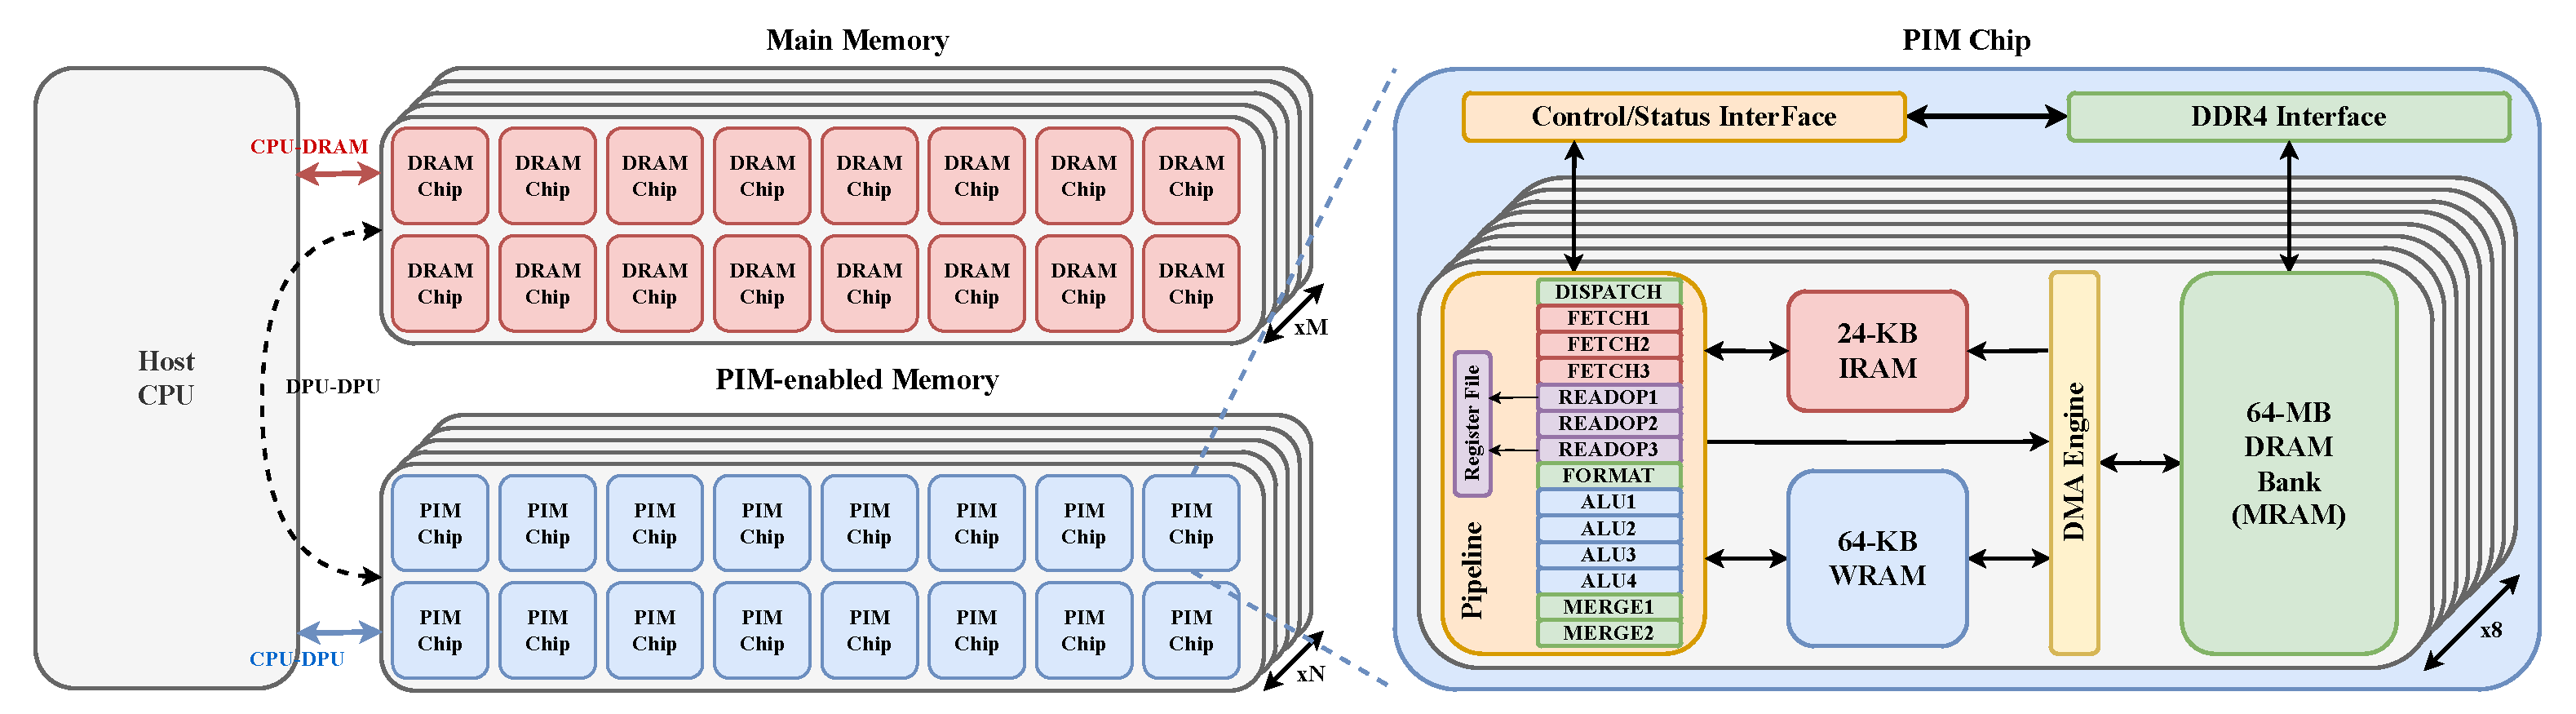
\includegraphics[width=0.9\textwidth]{figures/UPMEMArch.pdf}
    \caption{UPMEM硬件架构}
	\label{UPMEMArch}
\end{figure}

每个DPU拥有一个工作频率在400MHz的标量顺序(Scalar In-order)多线程的RISC核心,拥有16个物理线程和一个精调的(fine-grained)14级流水线。其中为了避免实现复杂的数据转发和流水线互锁电路 \cite{UPMEMHotChips},同一线程内的两个连续指令必须间隔 11 个周期才能被调度(只有最后三级ALU4、MERGE1、MERGE2可以和下一条指令的 DISPATCH、FFTCH 阶段并行执行)。因此至少同时有11个线程同时运行才能最大程度利用流水线。同时每个DPU的每个线程都有16个可用的32bit的寄存器,需要分奇偶访问。

UPMEM采取哈佛架构,将数据和指令分别存放,拥有24KB的指令存储器IRAM(能存放4096条48位指令)和64KB的数据存储器WRAM。DPU在工作时会在取指阶段访问IRAM,在访存和执行算术运算时访问WRAM。此外还存在存储层级MRAM,其就是每个DPU独占达的DRAM Bank,用于存放和CPU进行通信的数据,拥有较大的存储空间(64MB)。WRAM和MRAM除了在存储容量上的不同之外,由于WRAM本身属于静态RAM(Static Random Access Memory,SRAM),而MRAM就是正常的动态RAM(Dynamic Random Access Memory,DRAM),二者的访问速度存在着数量级的差别。再加上DPU无法直接访问MRAM需要通过WRAM进行中转,因此常规的访问方式是经过内置的DMA引擎将程序用到的大批量的数据从MRAM传输到WRAM中,再在WRAM中去频繁访存和计算。可以将WRAM视作通常意义上的Cache(工作缓存),而MRAM则类似于普通内存(数据主存),不同之处在于WRAM对开发人员不透明,需要手动管理。

UPMEM在硬件的基础上开发了一套完整的软件栈和工具链方便开发人员在其上搭建应用,包括DPU程序的运行时库、编译器,以及主机端调用DPU程序的API库,以及功能强大的调试器dpu-lldb。UPMEM的编程模式为单程序多数据(Single Program Multiple Data,SPMD)模型,DPU及其独占的bank相对于CPU来说类似于一个协处理器,CPU端被称为host端,而DPU端被称为device端。由CPU主动地将编译好的DPU程序装载入DPU并准备数据传输到DPU,再启动DPU执行程序,执行结束后收集结果或执行下一轮的任务。CPU和DPU之间的通信需要使用UPMEM提供的主机端API库,而DPU和DPU之间无法直接通信需要到CPU搬移到内存中进行中转。具体参数可以看表格\ref{UPMEMTable}。

\begin{table}[!htbp]
	\centering
	\label{UPMEMTable}
	\caption{UPMEM基本参数}
	\begin{tabular}{ll}
	  \toprule
	  名称 & 参数 \\
	  \midrule
	  Frequency & 400 MHz \\
	  Register width & 32 -bit (64 -bit support) \\
	  DPU-MRAM/DRAM Bandwidth & 1 GB/s \\
	  Threads & 16 \\
	  Main RAM (MRAM/DRAM) & 64 MB \\
	  Instruction RAM (IRAM) & 24 kB (4,096 $\times$ 48 -bit encoded instructions) \\
	  Work RAM & 64 kB \\
	  \bottomrule
	\end{tabular}
\end{table}

有许多工作对UPMEM的硬件特征做了系统且全面的测试\cite{BenchmarkingMutlu,BenchmarkingGermany,BenchmarkingUBC,BenchmarkingUPMEM,uPimulator},其中,Gómez-Luna等人\cite{BenchmarkingMutlu}的测试工作较为全面且权威。在这些评测中,不难发现UPMEM的硬件优势主要有下面几点:
\begin{itemize}
	\item [1)] 
	高存储容量和传输带宽,忽略WRAM等高速缓存,MRAM本身有64MB,2560个DPU共有160GB内存,远超市面上常用显卡的显存,每个MRAM的传输带宽大约为700MB/s,当2560个DPU并行工作其聚合带宽能够达到1.7TB/s,WRAM的聚合带宽更是能够达到6.8PB/s。      
	\item [2)]
	高并发和细粒度并发控制,如上所述,2560个DPU可以同时工作,每个DPU内部还可以控制16个线程进行更加细粒度的控制,虽然大多数测试中在跑常规测试集(Benchmark)时,超过11个线程并发就会让核心达到饱和,按照这个方式计算,整个PIM系统的并发线程数量能够达到近3万。
	\item [3)]
	高能效比,PIM设备由于减少了数据的多层级搬移可以大大降低能耗,文章\cite{BenchmarkingMutlu}中测试,UPMEM的能效比高于运行同等任务且优化成熟的CPU和GPU。
\end{itemize}

虽然UPMEM有上述的许多优点,作为商用近存计算硬件能够充分支持并行计算,但同时UPMEM的局限性也十分明显:
\begin{itemize}
	\item [1)] 
	UPMEM由于硬件资源十分有限,只支持32bit的整数加减法和8bit的乘法,其他的算术操作包括64bit的相关操作,乘除操作,浮点操作都是使用软件实现,效率较为低下;同时UPMEM本身主频不高,DPU处理器的规模受限,即使是32bit加法的MRAM计算访存比也只有1:4\cite{BenchmarkingMutlu},这些充分说明UPMEM的计算能力弱,更加适合内存瓶颈的任务。
	\item [2)]
	UPMEM的通信效率低,host和device的传输效率本身不高,只有大批量传输连续数据时才能勉强达到DDR4内存的传输带宽,同时DPU直接彼此独立缺乏有效的通信手段,只能通过CPU主动中转数据,效率更加低下。因此UPMEM不适合那些需要多核频繁通信的任务。\cite{BenchmarkingMutlu}。
\end{itemize}

\subsection{UPMEM相关应用}
自UPMEM可商用以来,有许多研究者就此硬件做出了许多工作。其中较为基础的一类是针对UPMEM硬件特征构建软件栈或对硬件做修改。如Khan等人\cite{CINMCompiler}针对包括UPMEM在内的诸多近存计算硬件构建了编译器,以支持开发人员在更高的抽象层级编程。同样的,Chen等人\cite{SimplePIM}也针对UPMEM硬件抽象更为高级的软件栈,包括对DPU的元数据管理、主从通信以及批处理模式三个大主要模块。同时,还有部分工作专注于拓展UPMEM基础软件库。Giannoula等人\cite{SparseP}开发了基于UPMEM的稀疏矩阵向量乘法(Sparse Matrix Vector Multiplication,SpMV)库,支持多种稀疏格式的矩阵以及数据格式,设计了多种数据映射和优化方法以适应不同的场景。Item等人\cite{TransPimLib}在UPMEM上开发了一套基于查找表(Look UP Table,LUT)和CORDIC (coordinate rotation digital computer)迭代的超越函数库,以一定的精度范围内支持了包括三角函数、指数对数、双曲线、平方根等复杂计算。Noh等人\cite{PID-Comm}针对UPMEM的DPU之间通信慢的问题,开发了一套支持多种通信模式的高效通信框架。除此之外,有部分工作在了解了UPMEM硬件的优缺点后,试图对UPMEM的硬件本身进行修改。北大的Zhou等人\cite{DIMM-Link}为解决UPMEM的通信慢的问题,增设外部数据连接电路联通物理相邻的DIMM,并设计数据转发和传输算法提高数据传输效率。

另外一大类重要的工作专注于利用现有UPMEM硬件去加速不同领域的应用,主要涉及到生物基因、数据库以及人工智能领域。生物基因领域主要是使用UPMEM加速基因测序和基因比对工作\cite{DNAMapping,VariantCalling,RNA-seq,UpPipe,GAPiM},这类工作的本质是字符串匹配为内存瓶颈任务,因此适合使用UPMEM硬件进行加速。数据库领域有许多工作对UPMEM关注密切。比如早期的工作\cite{Skyline}将skyline算子卸载到UPMEM。清华的Kang等人做了一系列的工作\cite{PIM-Model,PIM-Tree,PIM-Trie}将数据库常见的索引如跳表、前缀树的查询卸载到了UPMEM上,并充分设计了负载均衡算法保证查询速度。一些工作\cite{PIM-DB,PIM-Scan}将数据库最基本的查询算子,全部或部分卸载到了UPMEM上。Baumstark等人\cite{PIM—QueryCompile}将查询计划的优化也卸载到了UPMEM上。Lim等人\cite{PIM-Join}将数据库中的连接查询(Join)卸载到UPMEM上,通过巧妙地移位和排序解决了UPMEM因内存交错(Bank Interleave)带来的数据传输性能损失。

UPMEM的高并行和细粒度控制特性使得其非常适合用于AI和神经网络的场景。有相当一部分工作使用UPMEM加速神经网络的推理。Zarif等人\cite{UPMEMEmbeddingLookups}将UPMEM用于卸载巨大嵌入标的嵌入查找(Embedding Table Lookup)任务,加速效果尤为明显。Gómez-Luna等人\cite{UPMEMTraditionalML}将机器学习中经典的模型和算法卸载到了UPMEM上,包括线性回归、逻辑回归、决策树、K均值聚类,并对其分别测试了准确性、性能和扩展性,结果表明UPMEM相对于CPU有巨大提升,与GPU几乎持平。Das等人\cite{UPMEMCNN}在UPMEM上分别卸载了嵌入二值神经网络(Embedded Binary Neural Network ,eBNN)和高度量化的卷积神经网络YOLOv3,使用查找表消除乘除计算,这种极低bit量化在小模型上表现优异,但是不一定适用于大模型。Giannoula等人\cite{UPMEMGNN}将图神经网络(Graph Neural Network,GNN)的推理卸载到了UPMEM上,测试结果表明对于稀疏图和较为内存瓶颈的场景中,UPMEM的推理效率提升非常大。PIM-DL\cite{PIM-DL}使用UPMEM推理Bert,使用聚类算法构建向量乘以矩阵的查找表,通过对输入向量的子空间切分对查找表进行降维,从而消除GEMV算子为最近邻查找和向量加法,提高了计算效率。最近也开始有研究者尝试使用UPMEM加速神经网络的训练过程。Gogineni等人\cite{SwiftRL}提出SwiftRL以解决强化学习(Reinforce Learning,RL)中的内存瓶颈问题,将Tabular Q-learning和SARSA(State-Action-Reward-State-Action)等强化学习算法在UPMEM上实现,并适应不同应用场景。Rhyner等人\cite{PIM-Opt}希望在UPMEM实现分布式随机梯度下降算法(Stochastic Gradient Descent,SGD)探究UPMEM的AI训练能力和硬件特点。上述两个训练工作的结果都表明只有在内存瓶颈的应用场景下,UPMEM的训练性能提升较大,而且由于训练过程中存在跨节点通信,扩展性较差无法随数据规模线性扩展。

\section{本章小结}
本章首先详细地对大模型推理加速的技术和论文做了详尽介绍,从大模型的发展历程和模型结构的分析,了解大模型的推理成本很高,明白了加速推理的关键因素在于解决内存瓶颈或者提升基本算子的性能。随后介绍了模型量化的基本原理,以及用于加速大模型以缓解内存瓶颈的相关工作。然后对大模型推理阶段的基本算子矩阵向量乘做了基本介绍,并阐述了相关优化方法。本章还主要介绍了近存计算研究现状。首先梳理的近存计算的发展历程,包括近存计算的产生原因、发展和现状。然后着重介绍了第一款可商用的近存计算的硬件UPMEM,包括其硬件微架构和软件栈,同时结合相关测评工作说明了改硬件的基本特性。最后详细地介绍了基于UPMEM硬件上做的相关科研工作,涉及生物基因、数据库和机器学习等诸多领域,对研究现状有了充分的认识。